\begin{frame}{Quantifying  Separation}
	Possible Track Separation Variables
	\begin{itemize}
		\item $\Delta R_0$ : Separation between the electron and positron at the first tracking station in the x-y plane
		\item $\Delta X_0$ : Same as above but only in x direction 
		\item $\Delta Y_0$ : Same as above but only in y direction
		\item $\theta_0$ : Angle between the line connection decay vertex to the two tracks at the first tracking station
		% \item $\Phi_{p0}$ [To be Removed]
		\item $\Delta R_P = \sqrt{\Delta \eta ^2 + \Delta \phi^2}$  : Momentum space separation between electron and positron
	\end{itemize}
\end{frame}



\begin{frame}{Position Based Separation variables}
	\begin{figure}
		
	% Showing Various Separation
	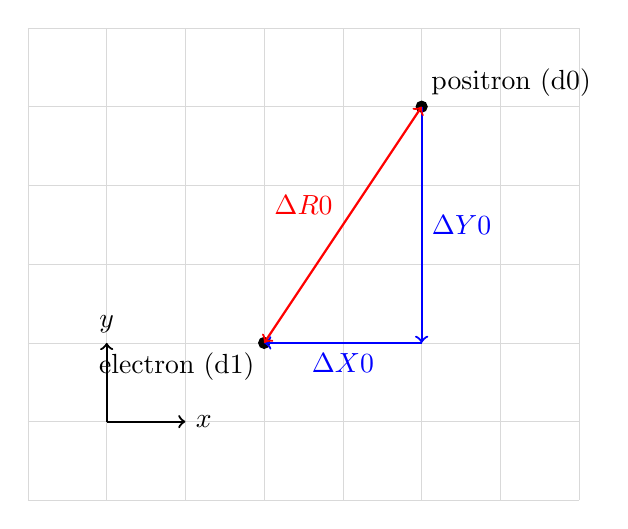
\begin{tikzpicture}[scale=1]
	% Draw grid
	\draw[step=1cm,gray!30,very thin] (-2,-1) grid (5,5);
	
	\coordinate (a) at (1,1);
	\coordinate (b) at (3,4);
	
	% Draw axes
	\draw[->,thick] (-1,0) -- (0,0) node[right] {$x$};
	\draw[->,thick] (-1,0) -- (-1,1) node[above] {$y$};
	% Mark Origin
	% \node[below right] at (0,0) {$(0,0)$};
	
	% Draw and label the points
	\filldraw (a) circle (2pt) node[below left] {electron (d1)};
	\filldraw (b) circle (2pt) node[above right] {positron (d0)};
	
	% Draw delta x, delta y
	\draw[->,thick,blue] (b) -- (a -| b) node[midway,right] {$\Delta Y0$};
	\draw[<-,thick,blue] (a) -- (a -| b) node[midway,below] {$\Delta X0$};
	
	% Draw delta r
	\draw[<->,thick,red] (b) -- (a) node[midway,above left] {$\Delta R0$};
	\end{tikzpicture}
	\caption{Tracking Station 1}
	\end{figure}

	ADD CODE SNIPPET
\end{frame}

\begin{frame}{Track Separation in terms of Angle}
	\begin{figure}
		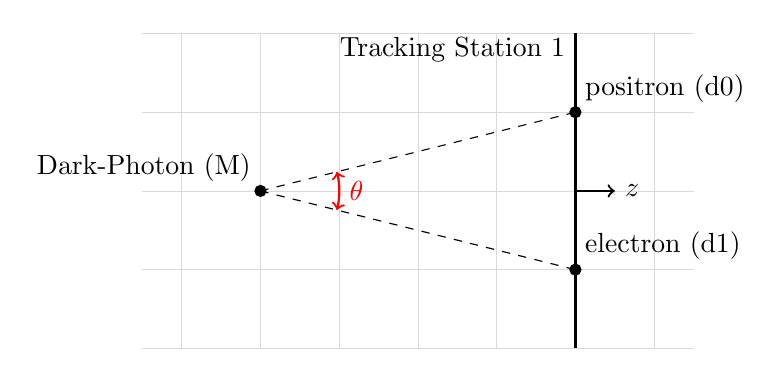
\begin{tikzpicture}[scale=1]
			% Define Mother and daughter particles
			\coordinate(M) at (-1, 0);
			\coordinate(d1) at (3, 1);
			\coordinate(d2) at (3, -1);
		
			% Draw grid
			\draw[step=1cm,gray!30,very thin] (-2.5, -2) grid (4.5, 2);
			\draw[-,thick] (3,-2) -- (3,2) node[pos=0.95, left] {Tracking Station 1};
			\draw[->, thick](3, 0) -- (3.5, 0) node[right] {$z$};
			
			% Draw mother and daughter particles
			\filldraw (M) circle (2pt) node[above left] {Dark-Photon (M)};
			\filldraw (d1) circle (2pt) node[above right] {positron (d0)};
			\filldraw (d2) circle (2pt) node[above right] {electron (d1)};
		
			\draw[dashed] (M) -- (d1);
			\draw[dashed] (M) -- (d2);
		
		% Draw arc and label the angle
		\draw[<->, thick, red] (M)+({atan(1/4)}:1) arc ({atan(1/4)}:{atan(-1/4)}:1) node[midway, right] {$\theta$};
		
		\end{tikzpicture}
		\caption{Angle between Tracks}	
		ADD CODE SNIPPET
	
	\end{figure}
	
\end{frame}

% \begin{frame}{Track Separation in terms of Momenta [Not Good]}
% 	\begin{figure}
% 	\begin{tikzpicture}[scale=1]
% 		% Define Daughter particles
% 		\coordinate(d1) at (3, 1);
% 		\coordinate(d2) at (3, -1);
	
% 		% Draw grid
% 		\draw[step=1cm,gray!30,very thin] (1, -3) grid (7, 3);
% 		\draw[-,thick] (3,-2) -- (3,2) node[pos=0.95, left] {Tracking Station 1};
% 		\draw[->, thick](3, 0) -- (3.5, 0) node[right] {$z$};
	
		
% 		% Daughter particles
% 		\filldraw (d1) circle (2pt) node[below left] {+ve charged (d0)};
% 		\filldraw (d2) circle (2pt) node[above left] {-ve charged (d1)};
	
% 		% Make Momentum Vectors
% 		\draw[->, thick, red]  (d1) -- ($(d1)+(1, 0.5)$) node[right] {$\vec{p_0}$};
% 		\draw[->, thick, blue] (d2) -- ($(d2)+(1, -0.5)$) node[right] {$\vec{p_1}$};
	
% 		% Show Translation
% 		\draw[dashed, red] (d1) -- (4, 0);
% 		\draw[dashed, red] ($(d1)+(1, 0.5)$) -- ($(4, 0) + (1, 0.5)$);
% 		\draw[dashed, blue] (d2) -- (4, 0);
% 		\draw[dashed, blue] ($(d2)+(1, -0.5)$) -- ($(4, 0) + (1,- 0.5)$);
	
% 		% Show angle between vectors
% 		\draw[->, thick, red] (4, 0) -- (5, 0.5) node[right] {$\vec{p_1}$};
% 		\draw[->, thick, blue] (4, 0) -- (5, -0.5) node[right] {$\vec{p_0}$};
% 		\draw[<->, thick] (4,0) + ({atan(-0.5/1)}:0.6) arc ({atan(-0.5/1)}:{atan(0.5/1)}:0.6) node[midway, right] {$\Phi_p$};
	
% 	\end{tikzpicture}
% 	\caption{Angle between Momenta}
% 	\end{figure}
% \end{frame}

\begin{frame}{Track Separation in $\eta$ - $\phi$ Space}
	\begin{figure}
	\begin{tikzpicture}[scale=1]
		% Define Daughter particles
		\coordinate(d1) at (0, 0);
		\coordinate(d2) at (0, 0);
	
		% Draw grid
		\draw[step=1cm,gray!30,very thin] (-1, -2) grid (3, 2);
		\draw[->, thick](-1, -2) -- (2.5, -2) node[right] {$\eta$};
		\draw[->, thick](-1, -2) -- (-1, 2) node[above] {$\phi$};
	
		
		% Daughter particles
		\filldraw (d1) circle (2pt); %node[below left] {+ve charged (d0)};
		\filldraw (d2) circle (2pt); %node[above left] {-ve charged (d1)};
	
		% Make Momentum Vectors
		\draw[->, thick, red]  (d1) -- ($(d1)+(1.5, 1)$) node[right] {$\vec{p_0}$ (d0)};
		\draw[->, thick, blue] (d2) -- ($(d2)+(1.5, -1)$) node[right] {$\vec{p_1}$ (d1)};
		\draw[<->, thick] (0,0) + ({atan(-1/1.5)}:0.6) arc ({atan(-1/1.5)}:{atan(1/1.5)}:0.6) node[midway, right] {$\Delta R_P$};
		
	
	\end{tikzpicture}
	\caption{Angle between Momenta}
	\end{figure}

\end{frame}

\begin{frame}{Code Sinppets}
	TODO: Fix listing here
% 	\begin{verbatim}
% 		XYZVector d0(truthd0_x[i], truthd0_y[i], truthd0_z[i]);
% 		Double_t deltaR = sqrt(pow(antimuon_at_station.X() - muon_at_station.X(), 2) + pow(antimuon_at_station.Y() - muon_at_station.Y(), 2));

% 		PxPyPzEVector d0(truthd0_px[i], truthd0_py[i], truthd0_px[i], truthd0_P[i]);
% 		Double_t deltaR = ROOT::Math::VectorUtil::DeltaR(antimuon_at_station, muon_at_station);
% 		XYZVector antimuon_at_station = d0_positions[1];
% 		XYZVector muon_at_station = d1_positions[1];

% 		Double_t deltaY = antimuon_at_station.Y() - muon_at_station.Y();
% 		Double_t deltaX = antimuon_at_station.X() - muon_at_station.X();
% 		Double_t deltaZ = (antimuon_at_station.Z() + muon_at_station.Z())*0.5 - (d0_positions[0].Z() + d1_positions[0].Z())*0.5;
% 		Double_t deltaR = sqrt(pow(deltaX, 2) + pow(deltaY, 2));
% 		Double_t theta = atan2(deltaR, deltaZ);
% 		\end{verbatim}
\end{frame}

\begin{frame}{Distribution of DeltaR0}
	\begin{figure}
		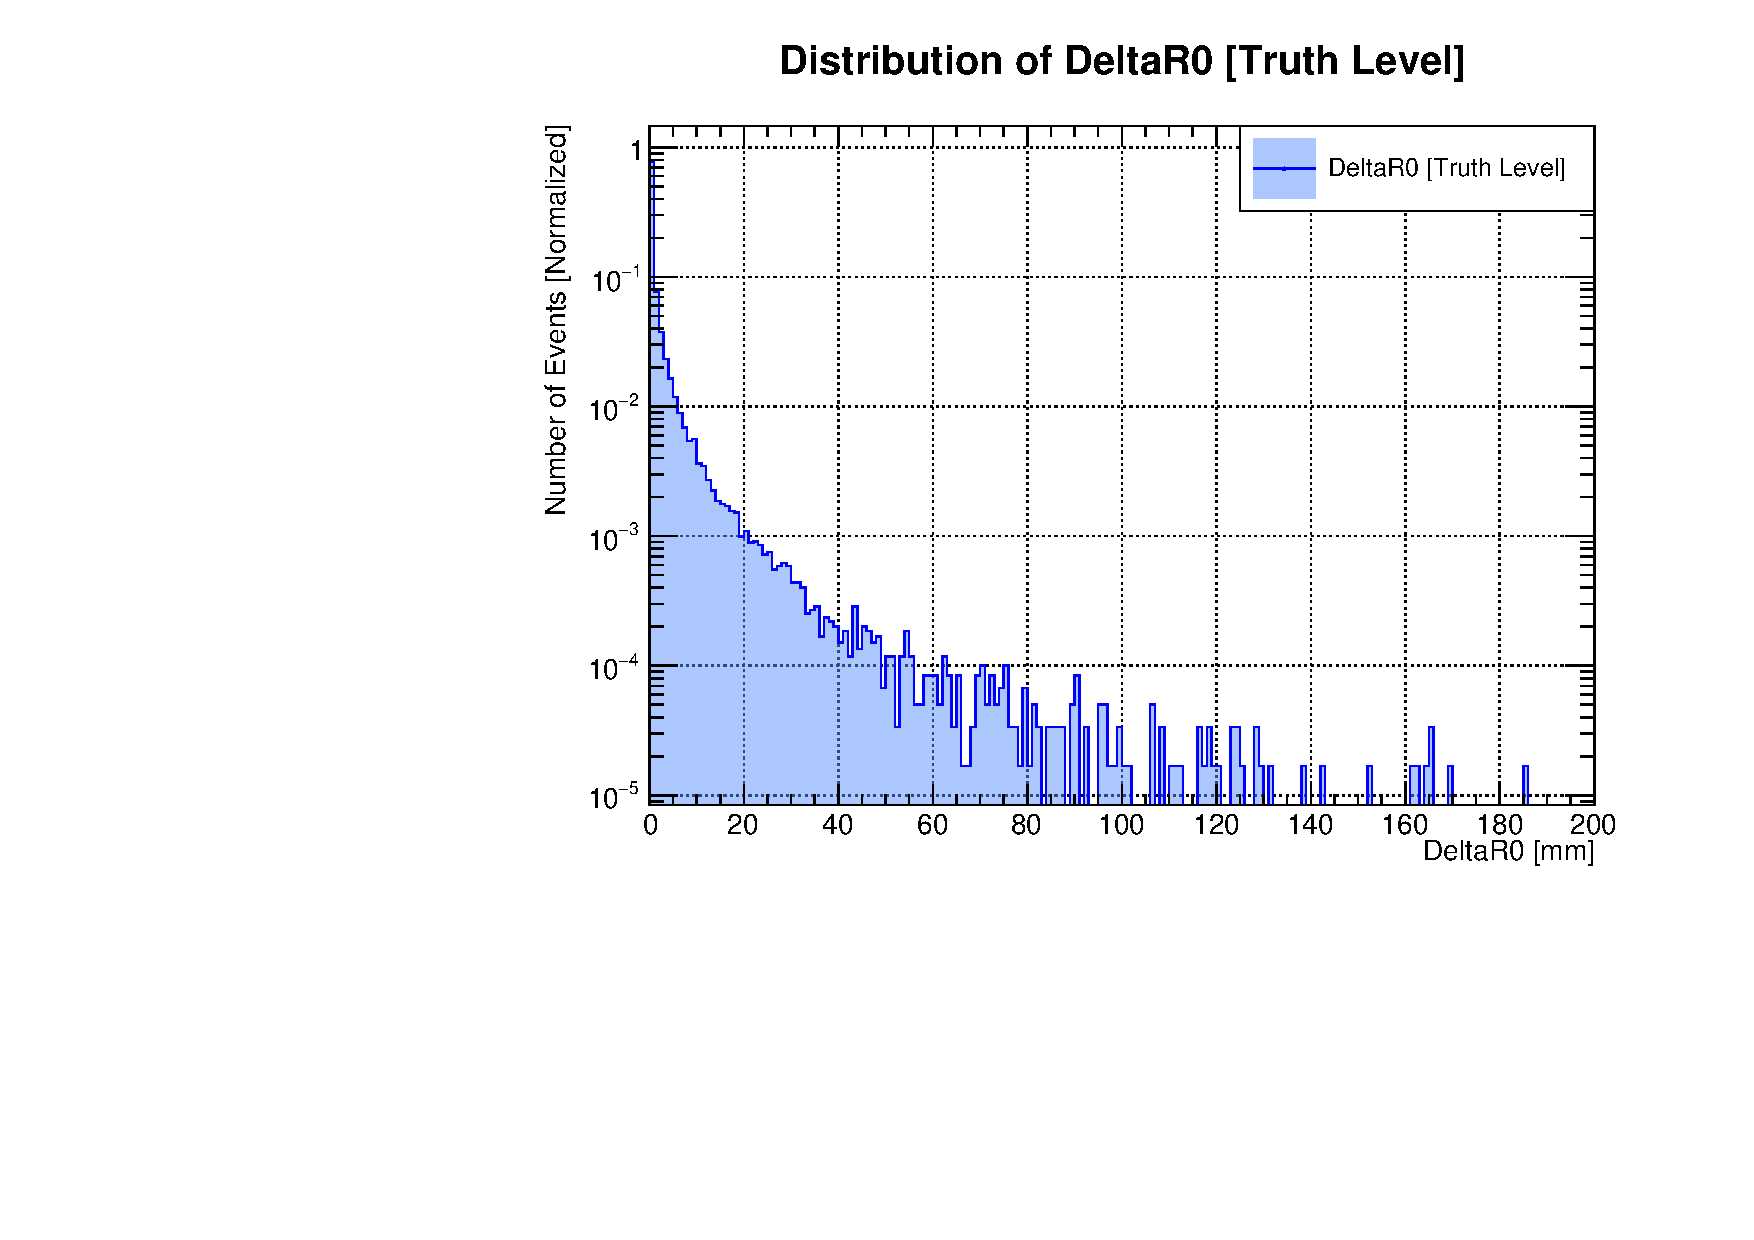
\includegraphics[width=\linewidth]{./output/DeltaR0.pdf}
	\end{figure}
\end{frame}

\begin{frame}{Distribution of DeltaX0}
	\begin{figure}
		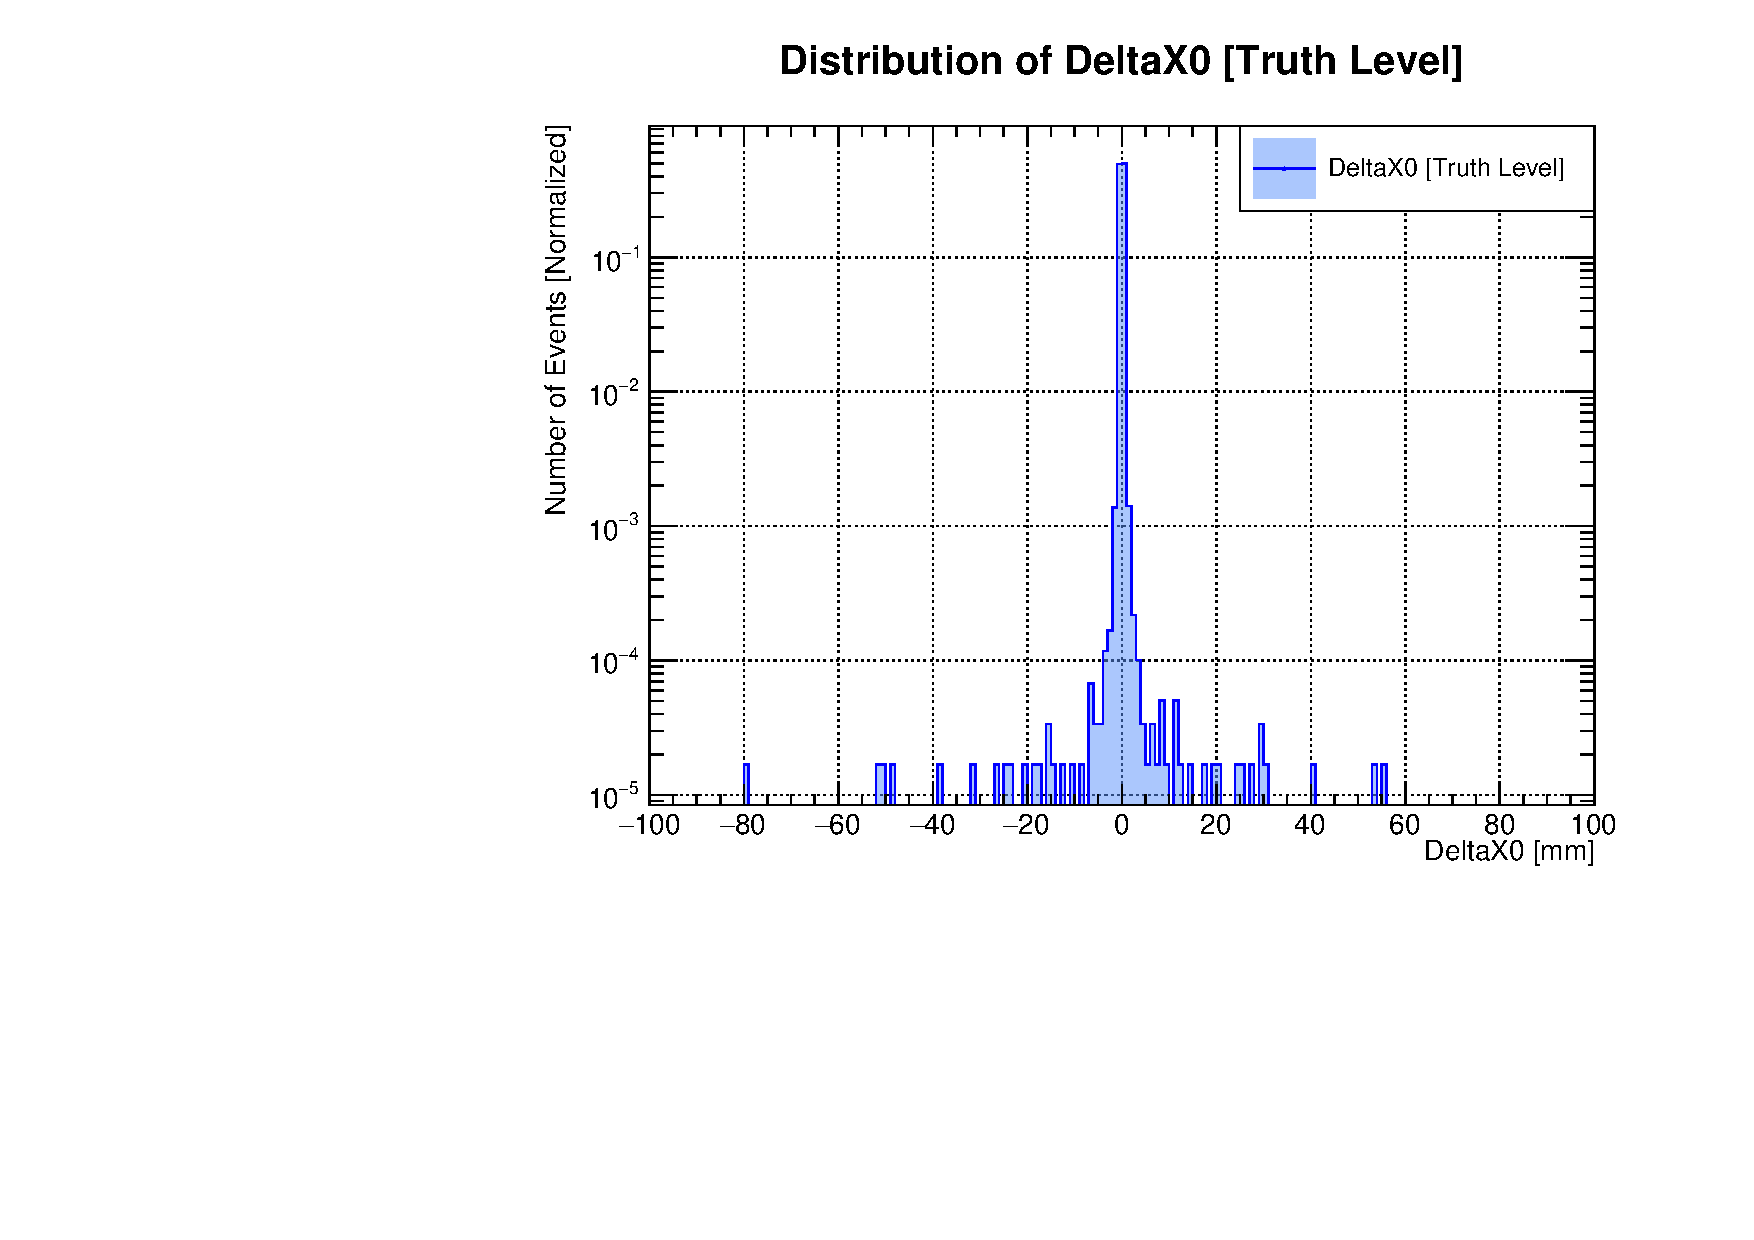
\includegraphics[width=\linewidth]{./output/DeltaX0.pdf}
	\end{figure}
\end{frame}

\begin{frame}{Distribution of DeltaY0}
	\begin{figure}
		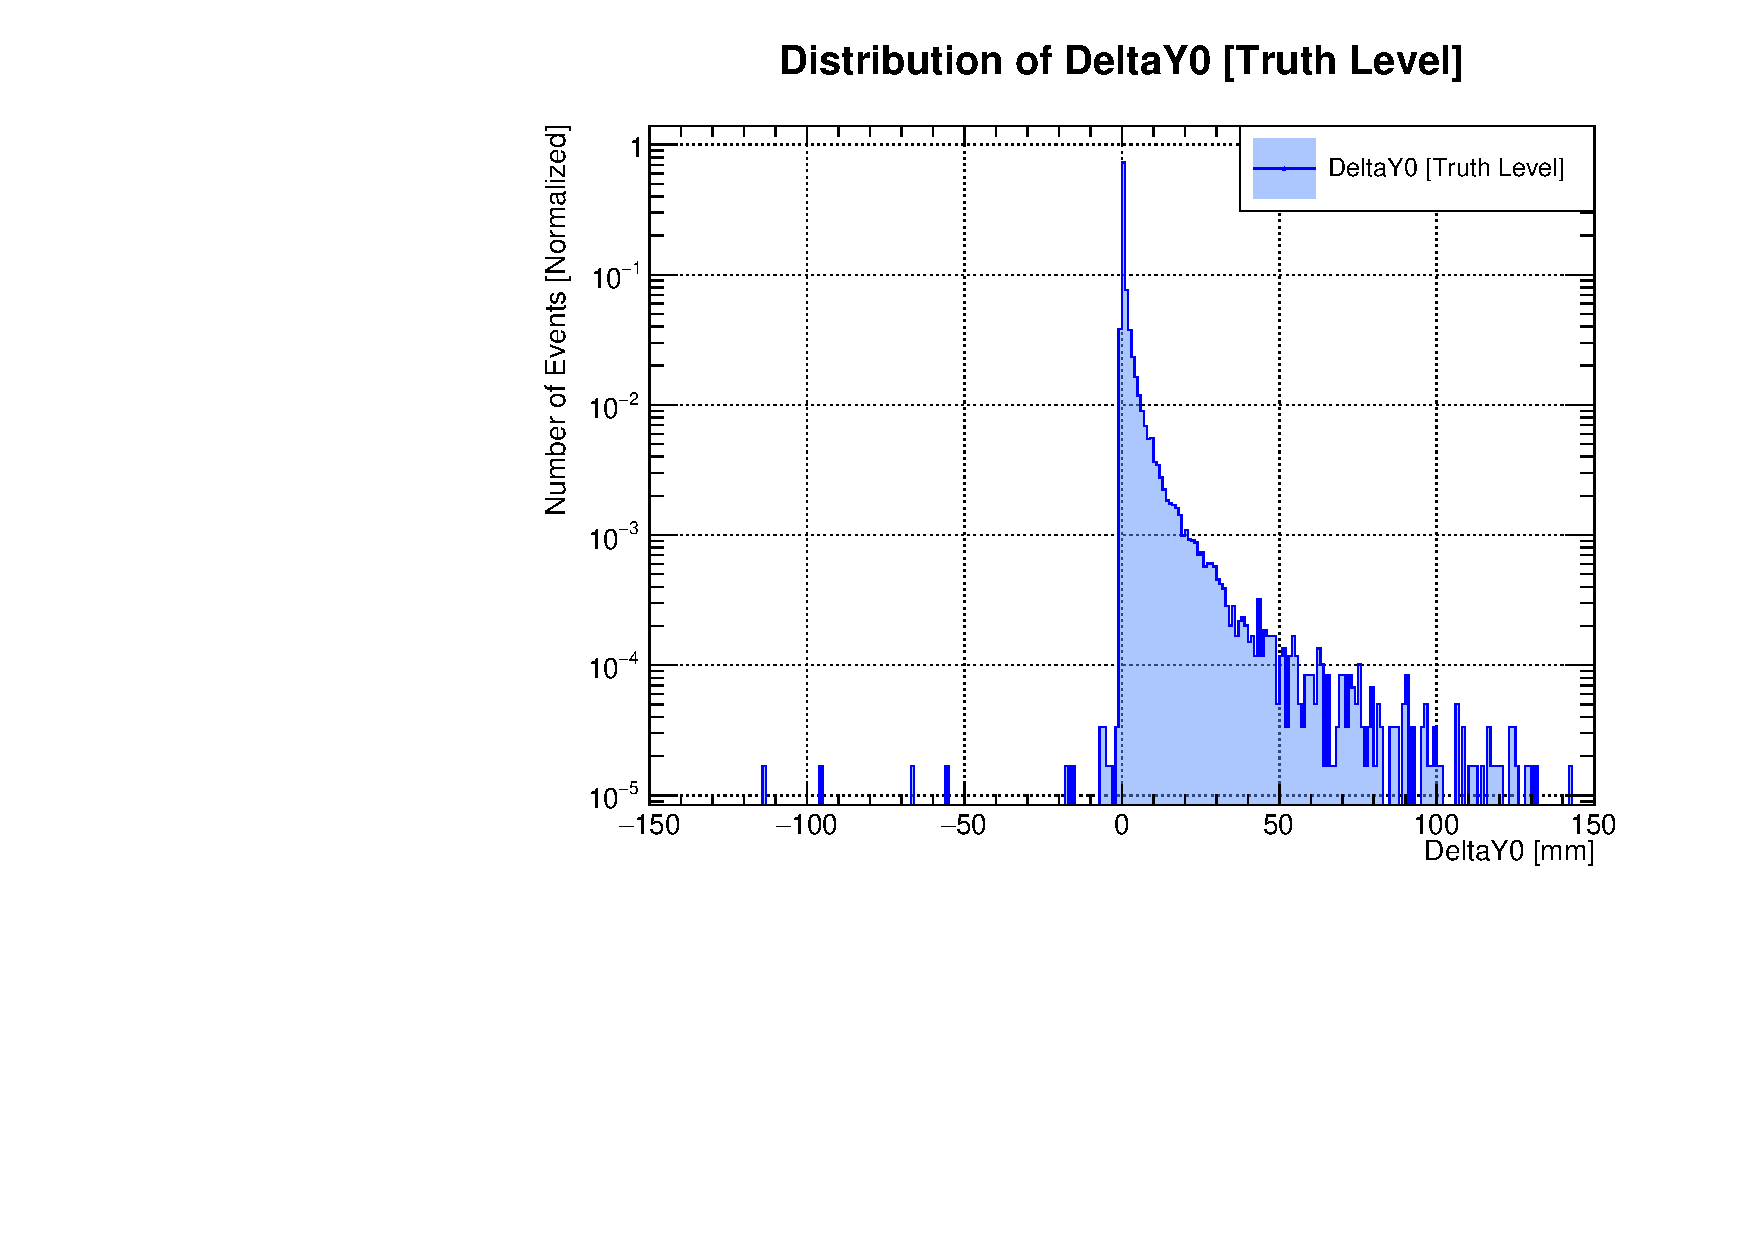
\includegraphics[width=\linewidth]{./output/DeltaY0.pdf}
	\end{figure}
\end{frame}

\begin{frame}{Comments on Position Based Separation}
		\begin{itemize}
			\item Particle predominantly separated in the y-direction
			\begin{itemize}
				\item Comes from the magentic field's deflection
				\item Positron deflected upwards, electron downwards leading asymmetry in DeltaY0 plot
				\item DeltaX0 looks symmetric
				\item DeltaY0 can be approximated to DeltaR0
			\end{itemize}
			\item In general Nevents fall off as sepration increases [characteristic of DP Decay?]
			\item Similar features seen in overlay plot but different in scale
			\item We can just look at the distributions using DeltaR0 as our primary variable for position based separation.
		\end{itemize}
		% \begin{figure}
		% 	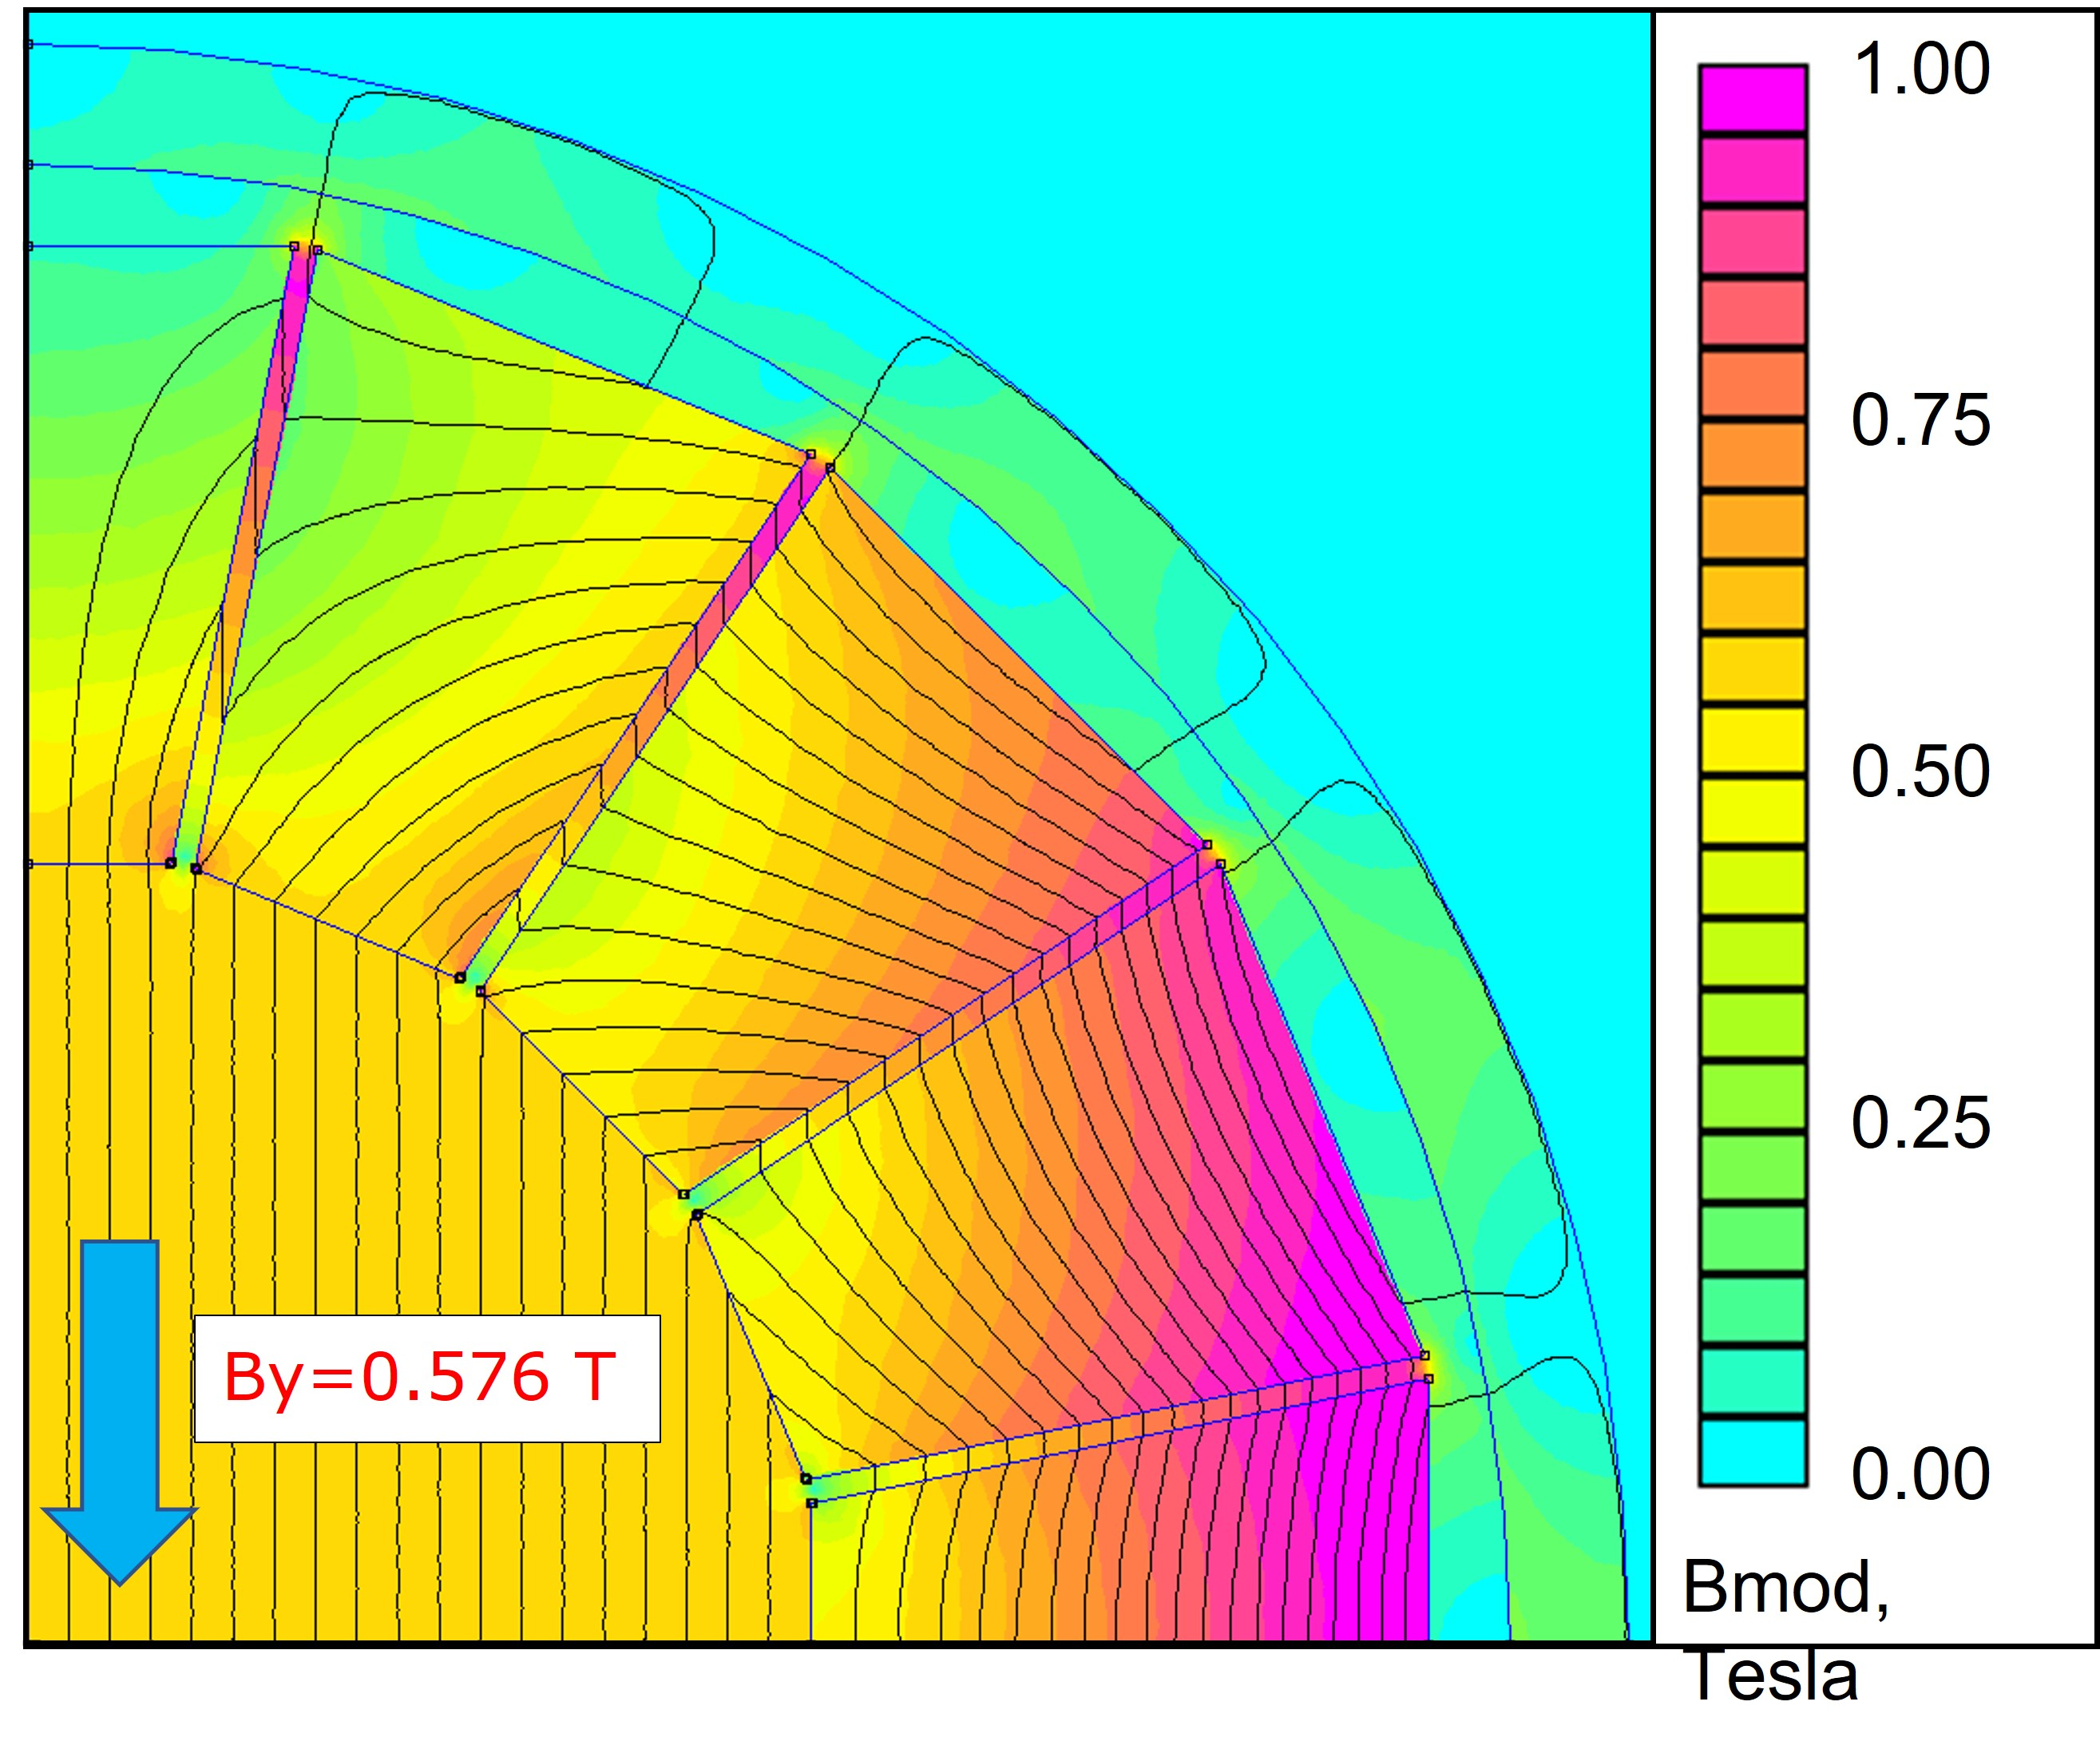
\includegraphics[width=0.5 \linewidth]{./assets/FASERMagField.png}
		% \end{figure}
\end{frame}

\begin{frame}{Overlay Plot}
	\begin{figure}
		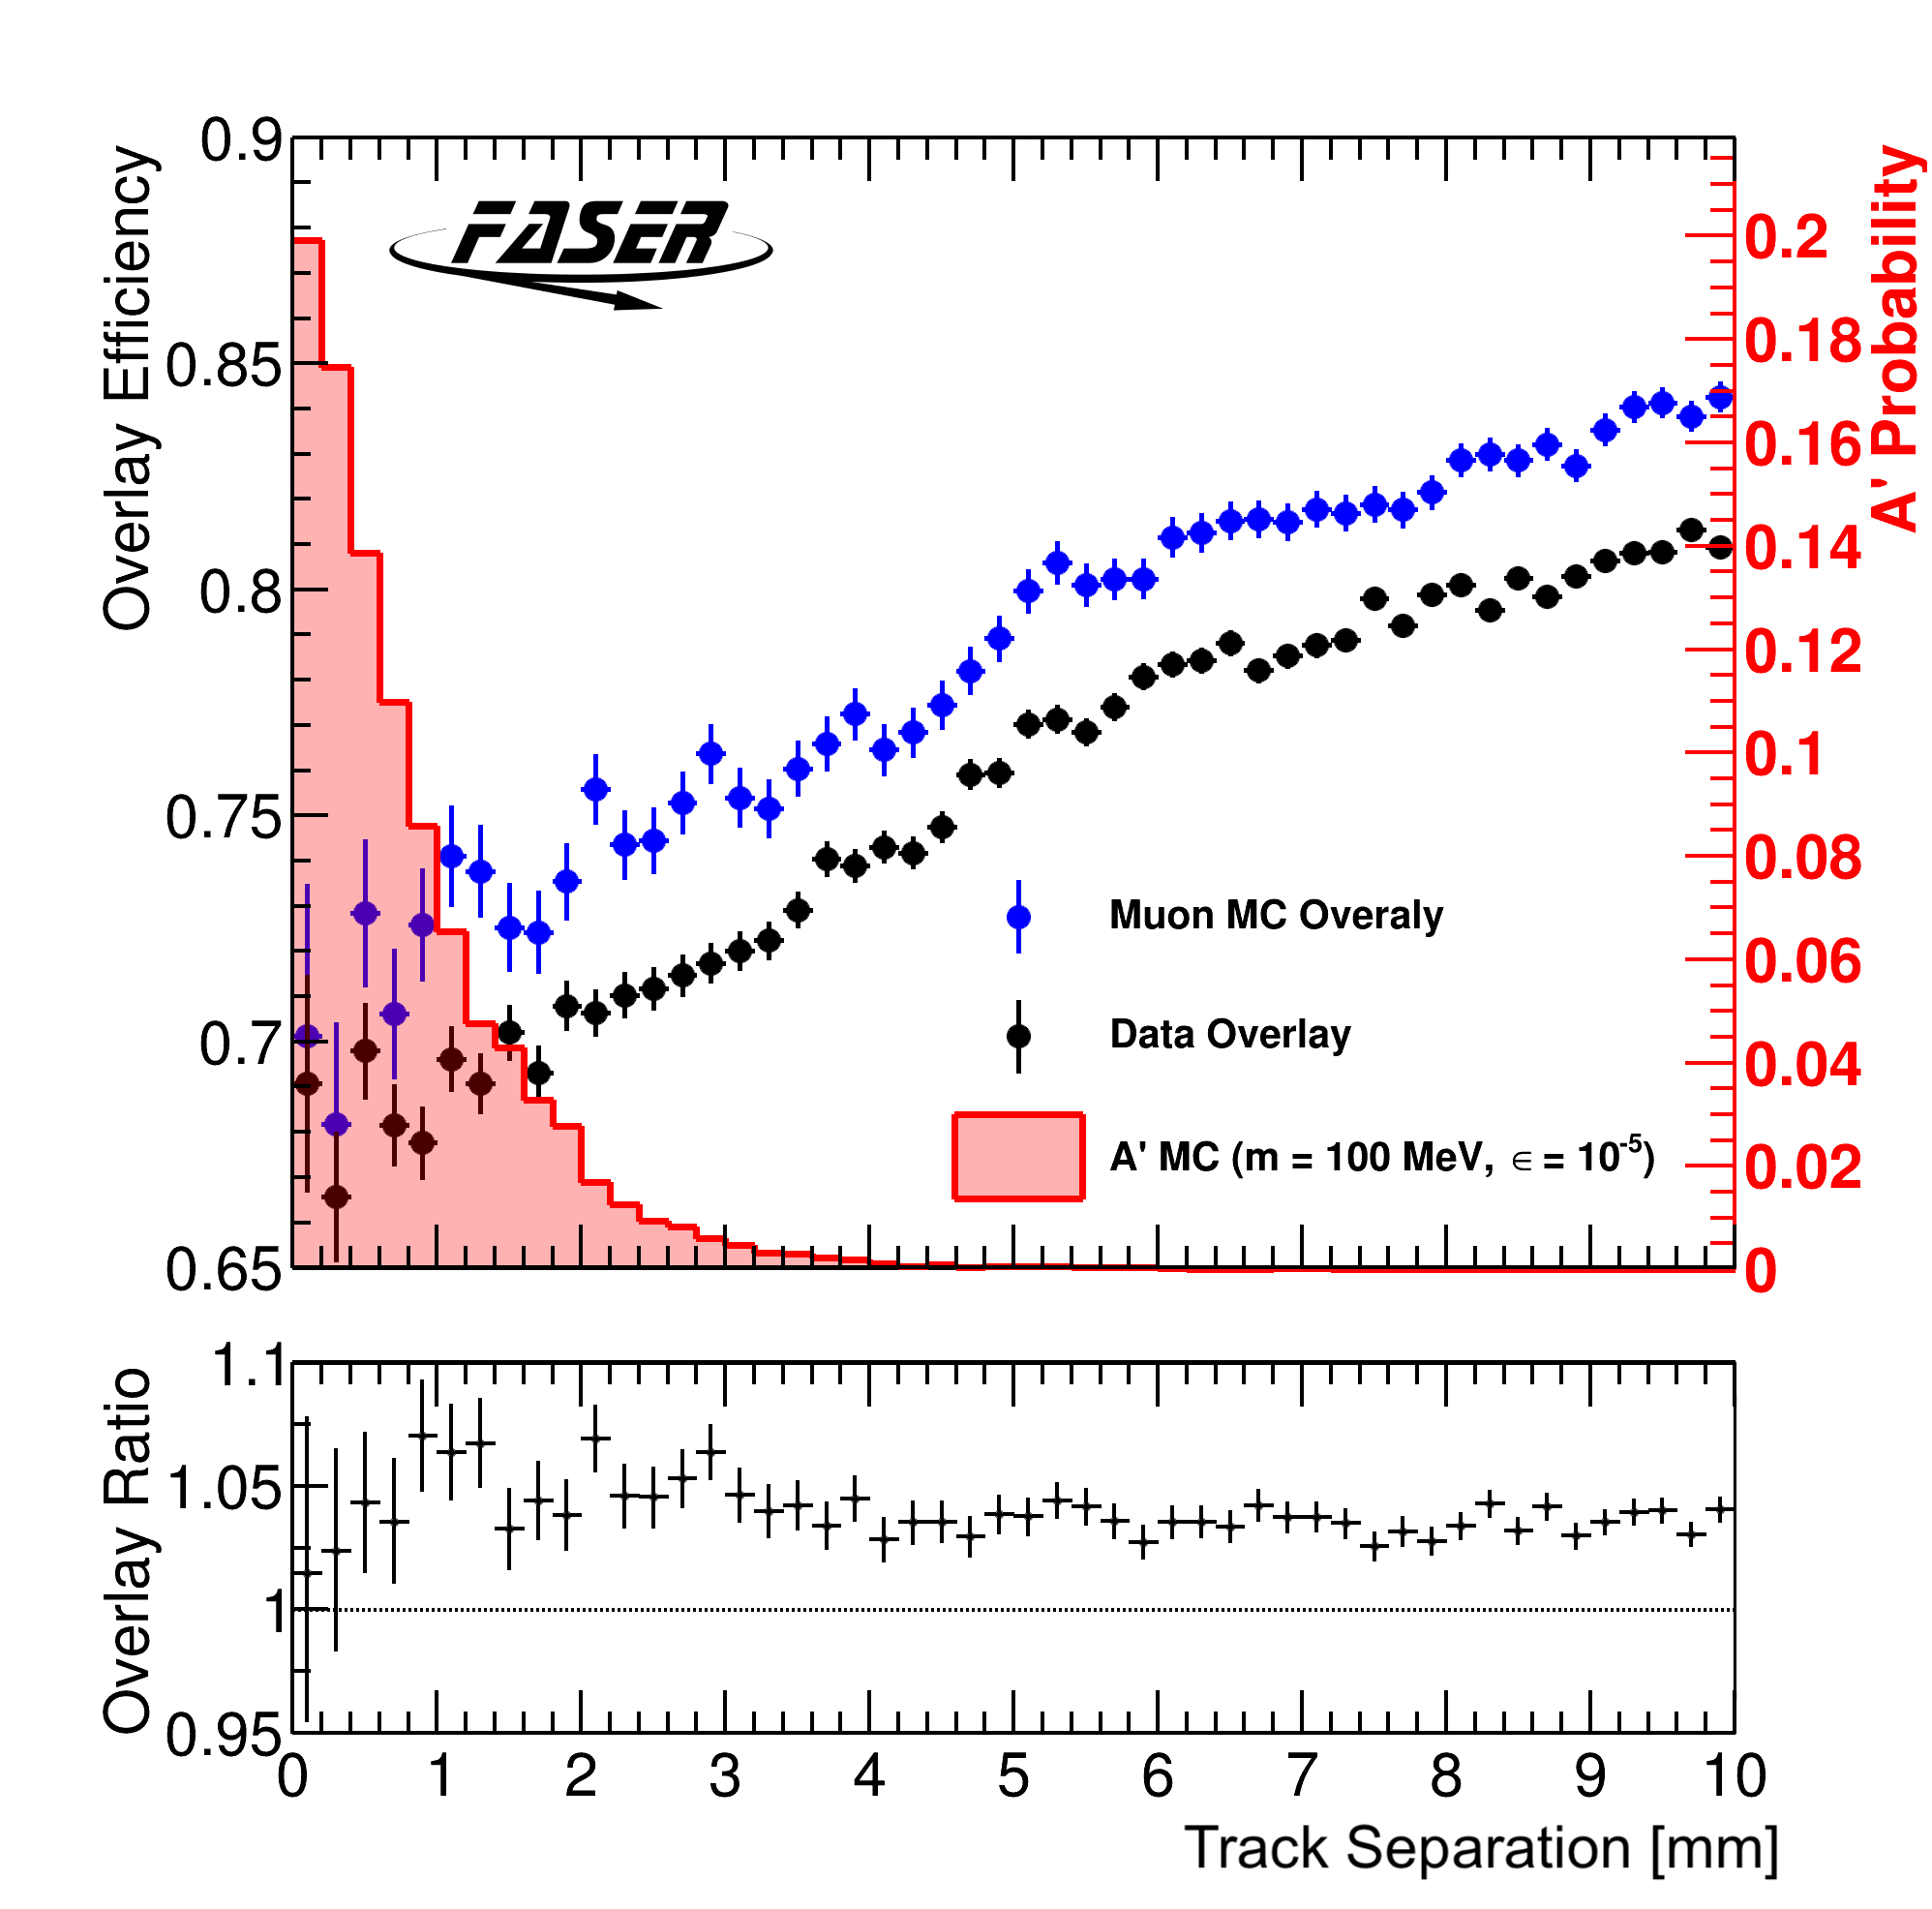
\includegraphics[width=0.7 \linewidth]{./assets/OverlayTracks.png}
		\caption{Overlay plot from \href{https://cds.cern.ch/record/2864686/plots}{Search for dark photons with the FASER detector at the LHC} }
	\end{figure}
\end{frame}

\begin{frame}{Distribution of Theta0}
	\begin{figure}
		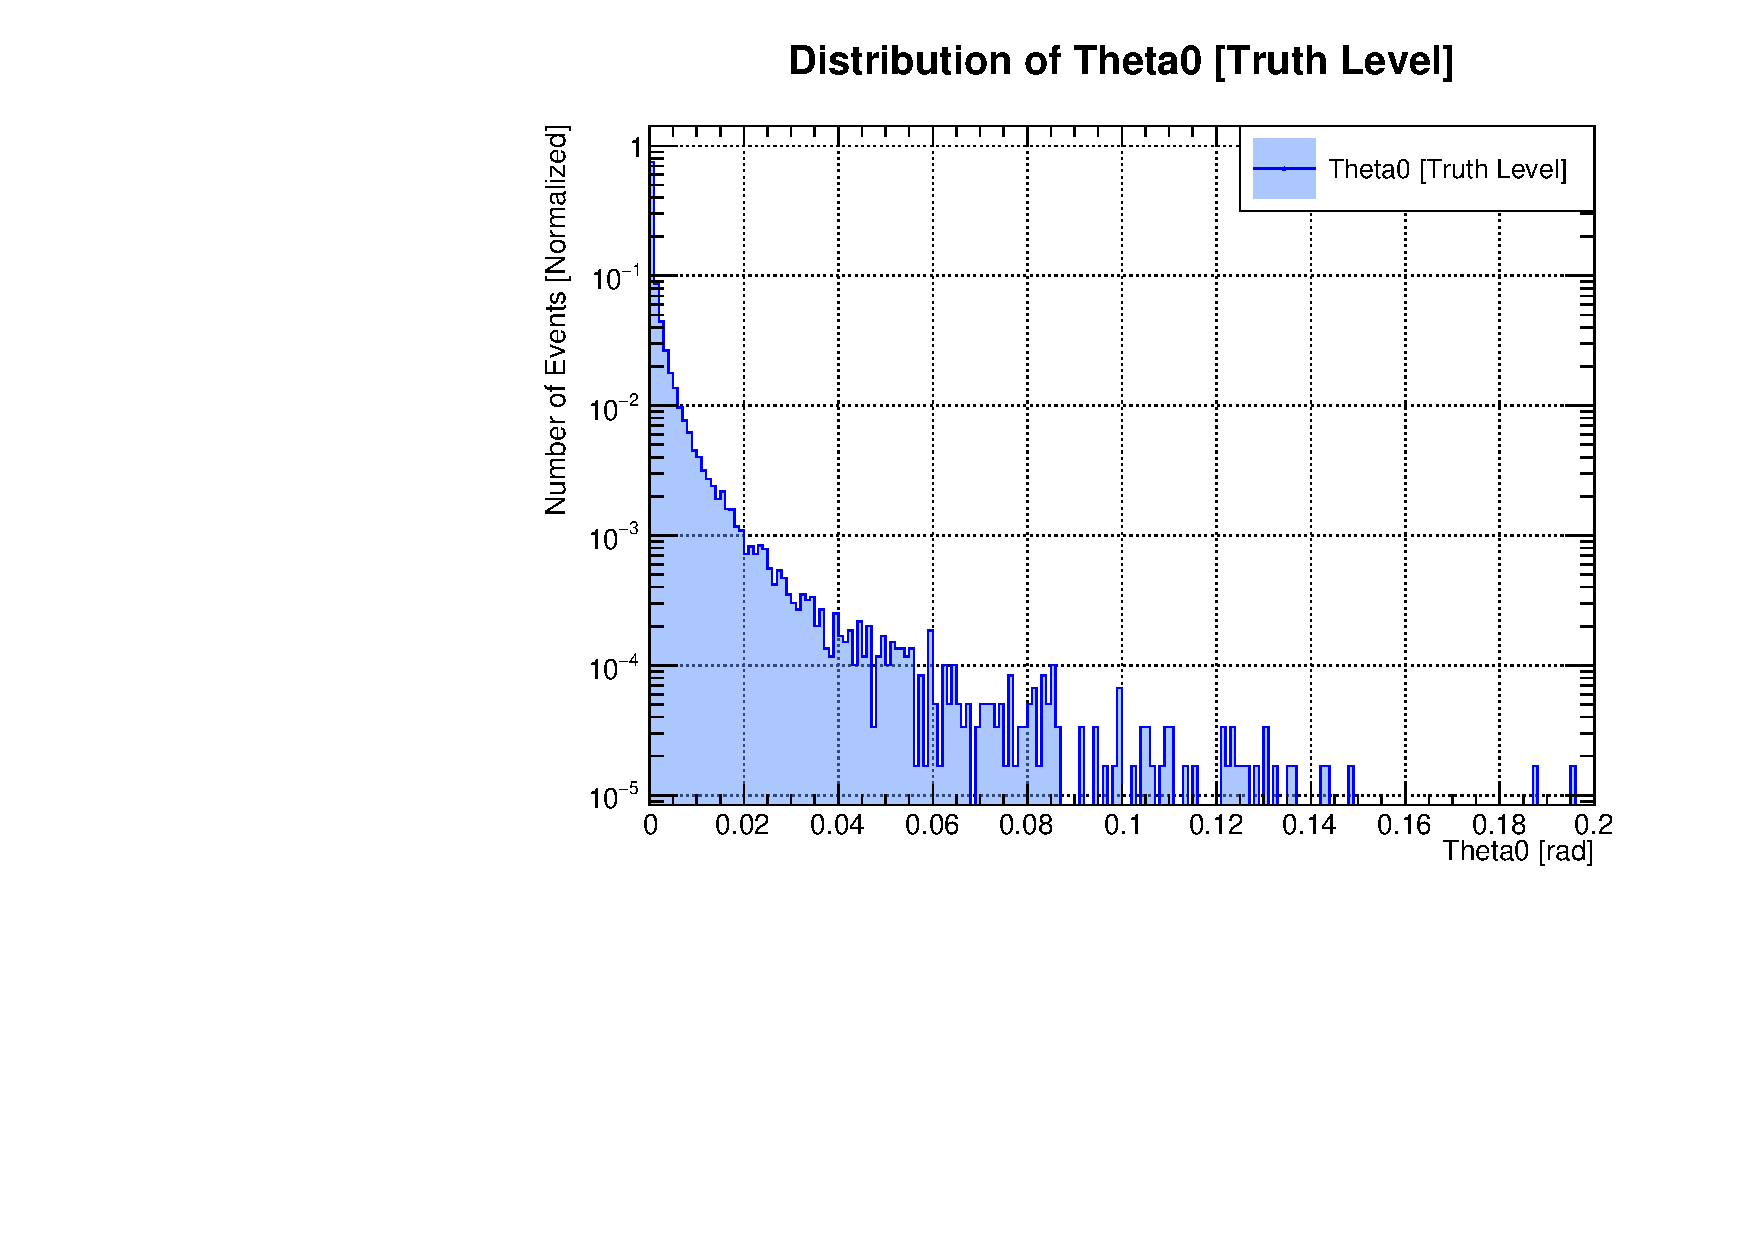
\includegraphics[width=\linewidth]{output/Theta0.pdf}
	\end{figure}
\end{frame}

\begin{frame}{Distribution of DeltaRP}
	\begin{figure}
		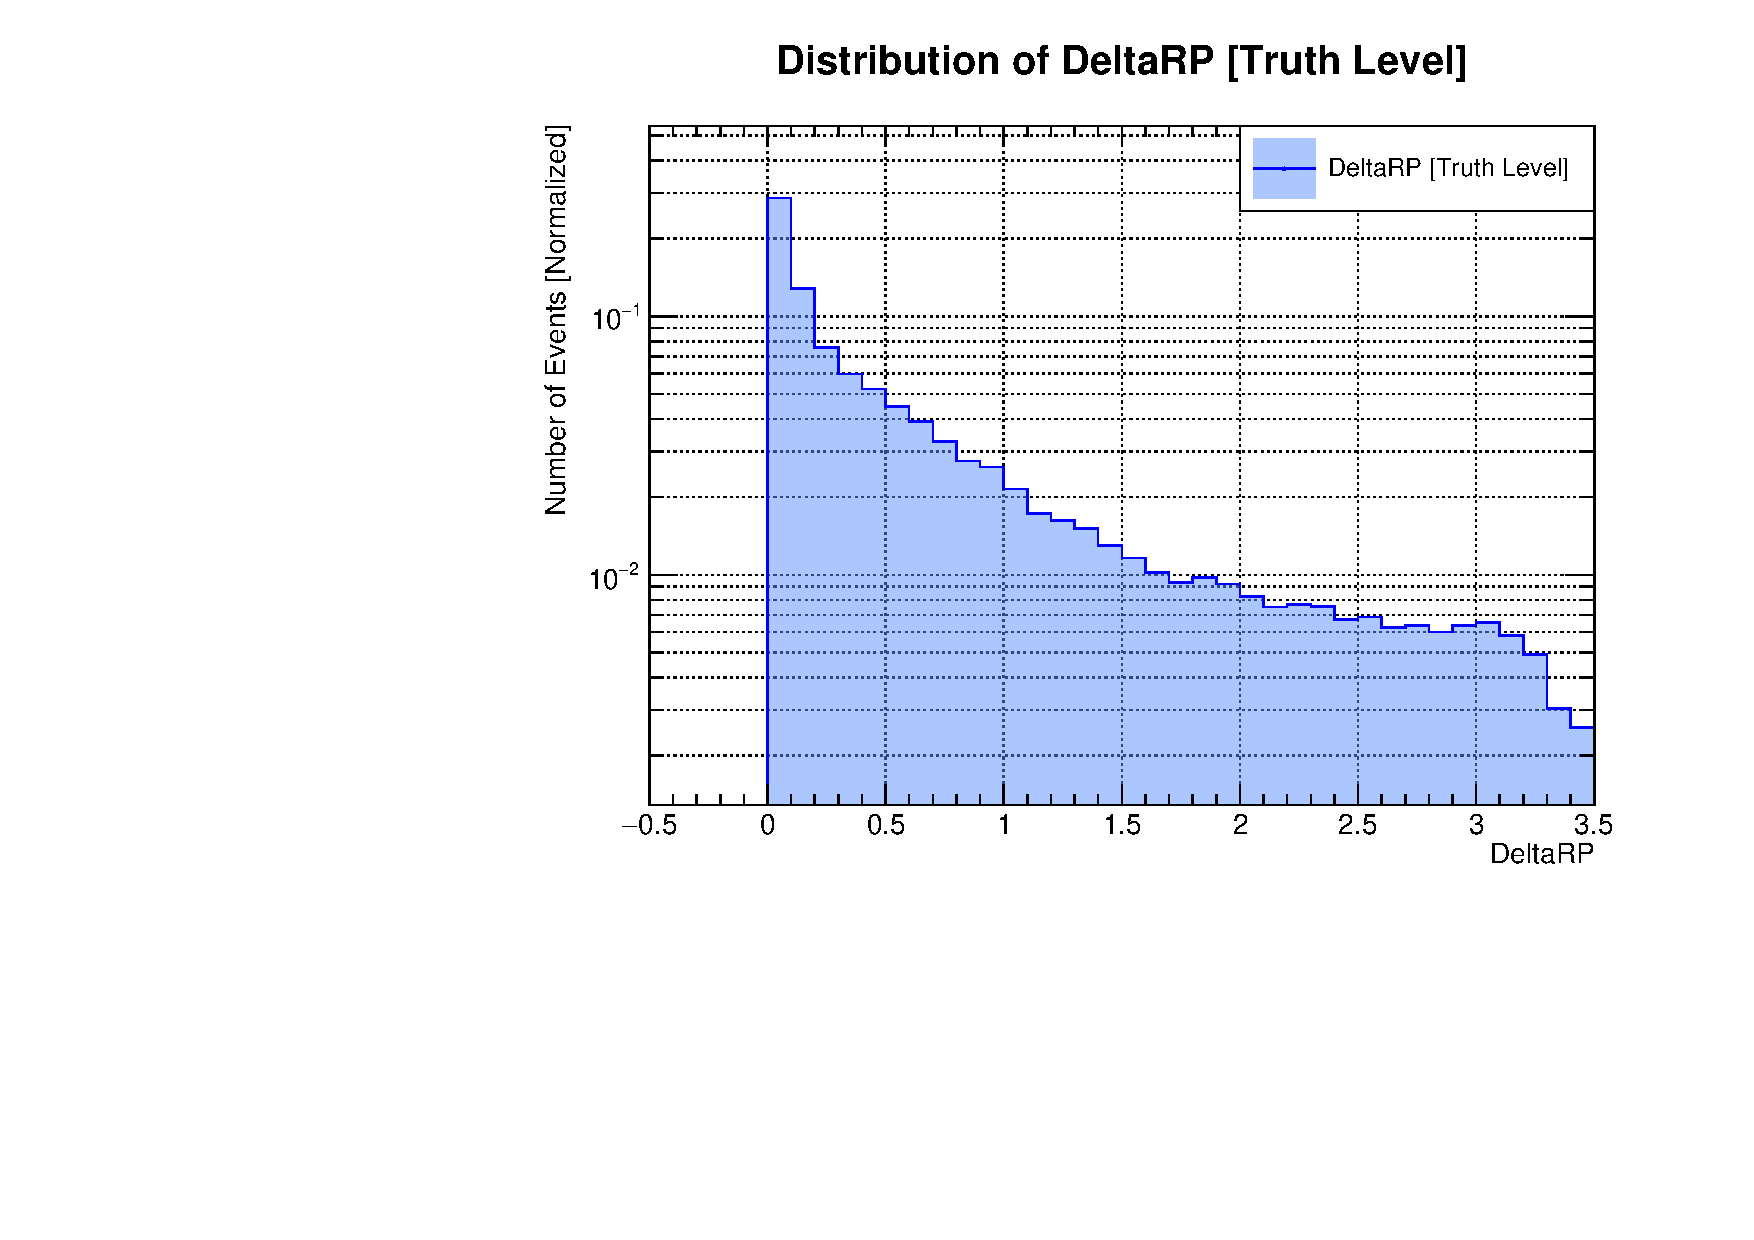
\includegraphics[width=\linewidth]{output/DeltaRP.pdf}
	\end{figure}
\end{frame}

\begin{frame}{Comments on Angle Based Separation}
	\begin{itemize}
		\item Theta0 is a variable to separate the tracks but falls off reapidly
		\item DeltaRP shows a relatively flat distribution
		% \item DeltaRP is a good variable to separate the tracks
		% \vspace{1 cm}
		\item To calculate the separation variables the MC level information is used
		\begin{itemize}
			\item Same across AL9 and CENTOS7
			\item More robust 
			\item No uncertainity from the tracking itself
		\end{itemize}
	\end{itemize}
\end{frame}